%%%%%%%%%%%%%%%%%%%%%%%%%%%%%%%%%%%%%%%%%%%%%%%%%%
%          Propiedades básicas del documento
%%%%%%%%%%%%%%%%%%%%%%%%%%%%%%%%%%%%%%%%%%%%%%%%%%

\documentclass [12pt, spanish] {article}
\usepackage [spanish] {babel}
\selectlanguage {spanish}

%%%%%%%%%%%%%%%%%%%%%%%%%%%%%%%%%%%%%%%%%%%%%%%%%%
%          Bibliotecas
%%%%%%%%%%%%%%%%%%%%%%%%%%%%%%%%%%%%%%%%%%%%%%%%%%

\usepackage {url} % Para introducir enlaces sin que se salgan de la página
\usepackage [utf8x] {inputenc} % Codificación de caracteres
\usepackage {graphicx} % Para incluir imágenes en el documento
	\graphicspath {{imagenes/}}
\usepackage {transparent} % Para la transparencia de la imagen de la portada
\usepackage {eso-pic} % Para colocar la imagen en la portada
	\AddToShipoutPicture* {
		\put(70,100) {
			\parbox [b] [\paperheight] {\paperwidth} {
				\vfill
				\centering {
					\transparent {0.1}
					\includegraphics [scale=2.2] {logo_ugr.png}
				}
				\vfil
			}
		}
	}
\usepackage{setspace} % Para el interlineado
\usepackage {parskip}
\usepackage {fancyhdr}
\usepackage {vmargin} % Marginado de la página
	\setmarginsrb {2 cm} {1 cm} {2 cm} {2 cm} {1 cm} {1.5 cm} {1 cm} {1.5 cm}
\usepackage [default] {sourcesanspro} % Fuente predeterminada

%%%%%%%%%%%%%%%%%%%%%%%%%%%%%%%%%%%%%%%%%%%%%%%%%%
%          Título, autores y fecha de compilación
%%%%%%%%%%%%%%%%%%%%%%%%%%%%%%%%%%%%%%%%%%%%%%%%%%

\title {
	Ingeniería, Empresa y Sociedad: \\
	The Walt Disney Company
	\hspace {0.05cm}
}
\author {
	Inés Nieto Sánchez \\
	Leire Requena García \\
	Clara María Romero Lara \\
	Atanasio José Rubio Gil
}
\date {\today}

\makeatletter
\let\thetitle\@title
\let\theauthor\@author
\let\thedate\@date
\makeatother

%%%%%%%%%%%%%%%%%%%%%%%%%%%%%%%%%%%%%%%%%%%%%%%%%%
%          Elementos de maquetación externos al cuerpo
%%%%%%%%%%%%%%%%%%%%%%%%%%%%%%%%%%%%%%%%%%%%%%%%%%

\pagestyle {fancy}
\fancyhf { }
\lhead {Ingeniería, Empresa y Sociedad: The Walt Disney Company}
\linespread{1.5}
\rhead {Universidad de Granada}
\cfoot {\thepage}

%%%%%%%%%%%%%%%%%%%%%%%%%%%%%%%%%%%%%%%%%%%%%%%%%%
%          Inicio del documento
%%%%%%%%%%%%%%%%%%%%%%%%%%%%%%%%%%%%%%%%%%%%%%%%%%

\begin {document}

	%
	%     Portada
	%

\begin {titlepage}
	\singlespacing
	\begin {center}
		\vspace* {8 cm}
		\textsc {INGENIERÍA INFORMÁTICA - UNIVERSIDAD DE GRANADA} \\
		{\huge \bfseries \thetitle} \\ [8 cm]
	\end {center}

	\begin {flushright}
		\large \theauthor \\ [0.973 cm]
	\end {flushright}

	\begin {center}
		\large \thedate
	\end {center}
\end {titlepage}

	%
	%     Índice
	%

\tableofcontents
\pagebreak

	%
	%     Secciones del trabajo (importadas desde archivos externos)
	%

\section{Introducción}

\pagebreak

\section{Misión, visión y propósito}

\pagebreak

\section{Propiedades de la empresa}

	\subsection{Tamaño}

Con un balance total de 98.598 millones de dólares y 201.000 empleados registrados el 30 de septiembre de 2018 (The Walt Disney Company, 2018), The Walt Disney Company se caracteriza indubitablemente como una empresa grande.
	\subsection{Sector}

The Walt Disney company se caracteriza por ser un conglomerado de decenas de empresas que operan en el sector del entretenimiento y de los medios de comunicación de masas. Internamente, ambos sectores están divididos en Walt Disney Studio Entertainment para las empresas dedicadas al entretenimiento, entre las que se encuentran Walt Disney Studio Motion Pictures, Marvel Enternainment, Hulu o la más olvidada The Muppets, y Walt Disney Television para aquellas del sector comunicativo, que recoge empresas de televisón como ABC, Disney Channel, Fox, o ESPN (The Walt Disney Company, 2015).

Por otro lado, debido a la gran cantidad de \textit{merchandising} que generan, sus productos ocupan una parte importante del mercado de productos de entretenimiento no cinematográfico, como pueden ser juguetes, ropa, videojuegos y parques de atracciones.
	\subsection{Ámbito geográfico}

Al tratarse de una empresa firmemente asentada en el sector de las industrias culturales, The Walt Disney Company opera globalmente en la distribución de productos audiovisuales, ya sean películas producidas por su estudio cinematográfico o programas emitidos en los canales de televisón que emiten a lo largo del planeta.

También cuentan con parques temáticos en California, Florida, París, Shanghai, Hong Kong y Tokio. A pesar de estar localizados en únicamente cuatro países, los parques de Estados Unidos cubren la demanda norteamericana; el francés, la europea; y los dos chinos y el nipón, la asiática.
	\subsection{Forma jurídica}
Disney se estructura como una sociedad anónima en la que cualquiera puede comprar acciones para invertir en la empresa.

	\subsection{Procedencia del capital}
The Walt Disney Company es una empresa de capital abierto desde en 1991 empezo a cotizar en bolsa vendiendo sus acciones. Es una empresa privada ya que su capital pertenece a los accionistas que han invertido en ella.
\pagebreak

\section{Planificación}

	\subsection{Objetivos estratégicos}
El gran tamaño de The Walt Disney Company hace que sea complicado dirigir la empresa. Para solucionar este problema, la compañía se encuentra dividida en empresas subsidiarias que se encargan de mantener el interés del público en sus respectivos ámbitos.

En cuanto a estrategia competitiva, The Walt Disney Company procura que la gente no abandone sus productos y, si alguna empresa les resulta un problema o es interesante para la mejora de sus productos, se planifica su compra para incorporarla a la compañía.
	\subsection{Objetivos tácticos}
Cada departamento de los anteriormente mencionados tiene sus propios objetivos tácticos.

Por ejemplo, en el sector cinematográfico, queda patente un claro objetivo táctico mantenido a lo largo del tiempo en la creación y publicación secuencial del llamado "\textit{Universo Cinematográfico de Marvel}", desde la compra de los derechos cinematográficos de la editorial de cómics, o la publicidad que se decide para sus películas con personajes originales.

Por otro lado, en el departamento de parques temáticos destaca el rescate que hubo que hacer en Disneyland París, que tiene pérdidas casi desde sus inicios (Pozzi, 2017). También son ejemplos la decisión de prohibir el consumo de alcohol en los parques o los eventos que se realizan en ellos.
	\subsection{Objetivos operativos}

	\subsection{Acciones planificadas}

	\subsection{Recursos}
The Walt Disney Company posee una gran variedad de recursos tangibles y intangibles.

Entre sus recursos tangibles podemos encontrar las oficinas, servidores, los edificios y atracciones que conforman sus parques, etc. Y entre los recursos intangibles tenemos por ejemplo, a todo el personal que trabaja en la empresa, el software que usan para sus películas de animación o los personajes que se encuentran en su propiedad intelectual.
	\subsection{Implantación del plan}

\pagebreak
	
\section{Organización}

	\subsection{Jerarquía de la empresa}
El actual presidente y CEO de The Walt Disney Company es \textbf{Robert Iger.} Bajo su mando directo se encuentra el equipo de gestión, compuesto por:
\begin{itemize}
\item Alan Braverman, consejero general, secretario y vicepresidente ejecutivo

\item Christine M. McCarthy, directora financiera y vicepresidente ejecutivo

\item Zenia Mucha, directora de comunicaciones y vicepresidente ejecutivo

\item Jayne Parker, directora de recursos humanos y vicepresidente ejecutivo

\end{itemize}

A excepción de Christine McCarthy, todos se encuentran al mismo nivel jerárquico. Ésta,  como directora financiera (CFO), supervisa la actividad global de la empresa.

Bajo esta organización, Disney se divide en cuatro grandes unidades empresariales. Cada rama se responsabiliza de su márketing y producción. Éstas son:
\begin{itemize}
\item Disney Media Networks, co-dirigida por James Pitaro y Peter Rice. Se encarga de el contenido y cadenas televisivas de Disney

\item Disney Parks, Experiences and Products, dirigida por Bob Chapek. Resorts, parques temáticos, actuaciones y merchandising.

\item Disney Studios Entertainment, co-dirigida por Alan Bergman y Alan Horn. Productora de todo el contenido audiovisual cinematográfico, musical y teatral.

\item Disney Direct-to-consumer and International, dirigida por Kevin Mayer. Conglomerado de servicios de streaming personalizados directos al consumidor

\end{itemize}

En estas ramas la organización se lleva a cabo en una estructura de organización funcional-lineal, desde los directores de unidad hasta cada empleado. 


	\subsection{Organigrama}

Contrariamente a la estructura jerárquica lineal propia de la gran mayoría de las corporaciones, The Walt Disney Company estructura su organigrama basándose en los procesos. De esta manera, se crea una red inminentemente sinérgica entre los diferentes sectores del núcleo de operaciones, que dependen de sus sectores colindantes y, a su vez, son dependencias del trabajo de ellos.

\begin{figure}[!htb]
	\centering
		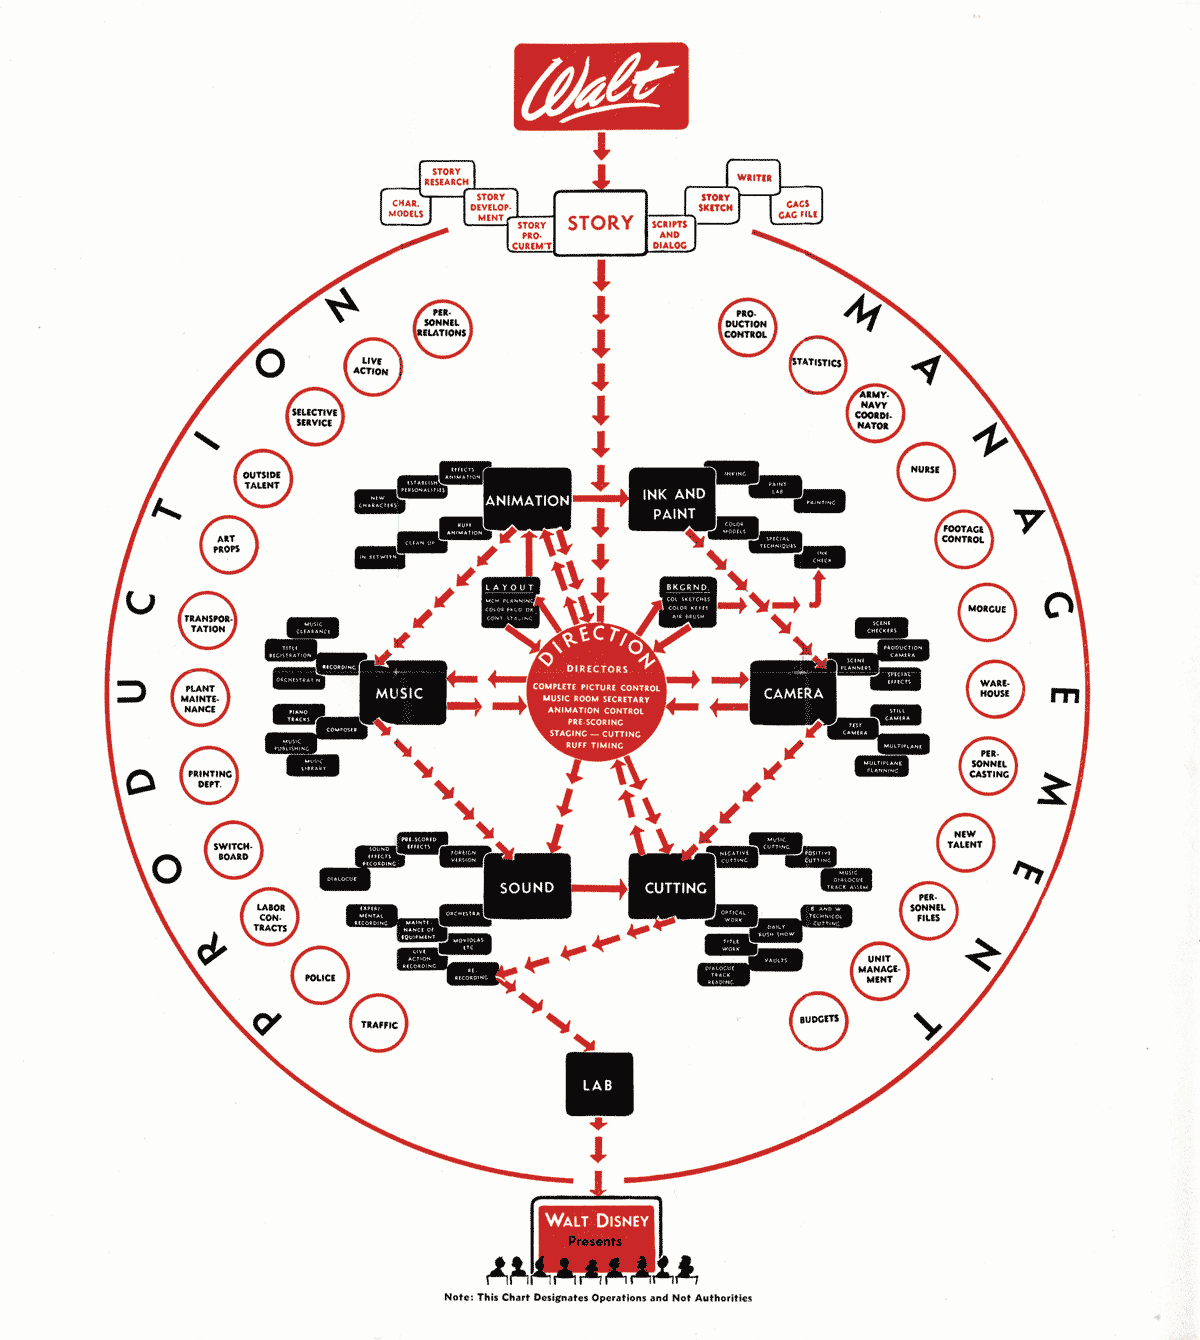
\includegraphics[scale=0.3]{organigramadisney.png}
		\caption{\label{fig:frog}Organigrama The Walt Disney Company (1943)}
\end{figure}

El organigrama más conocido de la empresa fue publicado en 1943 (Hirasuna, 2009) y muestra cómo cada una de las posiciones del staff son absolutamente necesarias para mantener activo el flujo del trabajo desde que la historia llega al equipo directivo cinematográfico desde los guionistas hasta que se lleva al público en la gran pantalla.
	\subsection{Responsabilidad social corporativa}

\pagebreak
	
\section{Dirección}

	\subsection{Propiedad de la empresa}
La propiedad legal de Disney pertenece a sus distintos accionistas, algunos de sus principales grupos son \textit{The Vanguard Group Inc.} o \textit{BlackRock Fund Advisors}.

Aunque los accionistas antes mencionados son grandes empresas, un individuo puede también poseer acciones de la compañía indica que el modelo que sigue es el anglosajón en el que las acciones se dividen en grupos amplios y variados.
	\subsection{Gobierno de la empresa}
Disney adopta políticas guvernamentales para prometer a sus stakeholders que sus negocios van a tener la máxima integridad. Por lo que cuenta con un Gobierno Corporativo que asegura esto y está formado por:

\begin{itemize}

\item
\textbf{Junta Directiva:} formada por líderes globales en la industria con grandes conocimientos y experiencia que permitirán la ganancia de valor a la compañía a largo plazo.

\item
\textbf{Comité de Auditoría:} su objetivo es preservar la integridad de los estados financieros, la adecuación de los sistemas de control, que se cumplan las normas establecidas y la independencia de los auditores independientes de la compañía.

\item
\textbf{Comité de retribuciones:} es el comité que informa a la Junta Directiva de The Walt Disney Company. Debe de hacer reviews y aprobar los objetivos corporativos y relevantes para la compensación del Director Ejecutivo y evaluar el desempeño del mismo. También ha de hacer recomendaciones a la Junta Directiva.

\item
\textbf{El Comité de Nominación y Estructura Corporativa:} revisa la correcta implementación y ejecución de las pautas del Gobierno Corporativo de la Compañía. También, identifica y revisa medidas para fortalecer el funcionamiento de las directrices del Gobierno Corporativo y aconseja a la Junta.

\item
\textbf{Comité Ejecutivo}

\end{itemize}
	\subsection{Dirección estratégica}
La dirección estratégica es la que vincula e inserta a la empresa en el mercado. Representa la dinámica de la empresa con su entorno y las acciones que lleva a cabo para lograr sus objetivos.

Para realizar una estrategia correcta para la empresa tenemos que analizar el entorno interno y externo con el análisis DAFO y el específico con las 5 Fuerzas del Diamante de Porter.
		\subsubsection{Análisis del entorno interno y externo}

Siendo la empresa más importante de todo el mundo en el sector del entretenimiento y de los medios de comunicación de masas, The Walt Disney Company se caracteriza por tener un gran asentamiento en la industria y una relación simbiótica con el resto de empresas, que no pueden competir directamente contra ella. A su vez, su dominante posición en una industria le permite moverse hacia nuevos horizontes, como hicieron con la creación del primer parque de atracciones.

Sin embargo, su clara posición también juega un papel en su contra, ya que cualquier cambio en la tecnología o el producto puede presentar una alteración importante de la imagen. Por otro lado, debido a que opera en el sector de las industrias culturales, la obtención ilegal de sus productos o el cambio de los gustos de su público objetivo son amenazas contra las que debe estar siempre atenta.

\begin{table}[]
\centering
\begin{tabular}{rl}
\textbf{DEBILIDADES} & \textbf{AMENAZAS} \\
Innovación limitada & Competencia cultural \\
Diversificación limitada & Rupturas tecnológicas \\
Expansión de parques limitada & Piratería del contenido digital \\
\textbf{FORTALEZAS} & \textbf{OPORTUNIDADES} \\
Popularidad de la marca & Innovación tecnológica \\
Cartera de productos creciente & Crecimiento en diferentes industrias \\
Fuerte crecimiento cooperativo & Crecimiento en mercados en desarrollo \\
\end{tabular}
\caption{\label{fig:frog}Análisis DAFO de The Walt Disney Company (Brown, 2017)}
\end{table}
		\subsubsection{Análisis del entorno específico}
Como se ha mencionado anteriormiente, The Walt Disney Company opera en el sector del entretenimiento y los medios de comunicación de masas. Siguiendo el modelo de Porter del diamante de cinco fuerzas, podemos encontrar las siguientes:

\begin{itemize}

\item
\textbf{Fuerza 1 - Amenaza de nuevos competidores:} The Walt Disney Company tiene previsto introducirse en el servicio del \textit{streaming}, convirtiendo a empresas como Netflix y HBO en sus nuevos competidores. En cuanto al mundo cinematográfico, existen competidores ya establecidos como DreamWorks, Nickelodeon y WarnerBros.

\item
\textbf{Fuerza 2 - Intensidad de la rivalidad entre competidores existentes:} Como se ha mencionado anteriormente, The Walt Disney Company tiene una relación simbiótica con las empresas, lo que permite eliminar gran parte de la competencia, y está tan establecida que apenas tiene competencia. En caso de tenerla, adquiere a la compañía que pueda causarles perjuicios económicos, como es el caso de Fox (Gartenberg, 2017).

\item
\textbf{Fuerza 3 - Productos sustitutos:} En este caso cualquier otra empresa dedicada al entretenimiento infantil como lo son Boing o Clan Tv es un producto sustituto de Disney. SixFlags o SeaWorld son, por otro lado, parques temáticos sustitutos de Disneyland. No obstante, las amenazas de productos sustitutos es baja debido a la distinción de la marca y su imagen.

\item
\textbf{Fuerza 4 - Poder negociador de los clientes:} Debido a la popularidad de la marca y la diferenciación de los productos que ofrece, el poder de negociación de los clientes es débil, lo cual ha incrementado la lealtad de los mismos. Esto se ha podido reflejar en la subida de precio en las entradas de sus parques temáticos y la apenas inexistente pérdida de visitante a causa de ello.

\item
\textbf{Fuerza 5 - Poder negociador de los proveedores:} La integración vertical de Disney reduce el poder negociador de los proveedores. La compañía se caracteriza por la alta calidad de sus productos, por lo que los proveedores deben de comprometerse a ofrecer productos con las características esperadas, ya que en caso contrario son rápidamente reemplazados.

\end{itemize}
	\subsection{Dirección de producción}

		\subsubsection{Proceso de producción}
La creación de un nuevo producto en Disney comienza con un brainstorming, es decir, una lluvia de ideas del proyecto que se va a comenzar. En esta etapa se busca encontrar aquella idea que sea la mas creativa y con ello la más diferenciada que aporte el máximo beneficio posible.

Walt Disney tenía su propio método, llamado Imagineering (Ingeniería de la imaginación). Este contaba con tres fases: la del soñador (asocida al brainstorming mencionado anteriormente), realista y crítico. Con ellas conseguía elegir las mejores ideas y contestar a las siguientes preguntas:

\begin{itemize}

\item
\textbf{El soñador, ¿a dónde podemos ir?:} en esta fase se deja volar la imaginación, sin tener límites y sin forzar a que una idea sea realista.

\item
\textbf{El realista, ¿cómo podemos llegar ahí?:} Es el que se cuestiona si una idea es realizable o no, intenta comprender cómo hacer lo que en la etapa anterior hemos propuesto sin tener límite alguno.

\item
\textbf{El crítico, ¿se puede llegar?:} busca las debilidades y desmonta argumentos que en caso de fallar en ello indica que se trata de una buena idea, la cual puede convertirse en un producto final de éxito.

\end{itemize}
Estas fases debían de estar aisladas las unas de las otras, pues consideraba que el realismo no podía interferir en la primera fase que era la más creativa.

No obstante, no hemos de olvidar otros factores importantes como lo son la comunidad, la colaboración y el buen hacer de los trabajadores.


		\subsubsection{Ciclo de vida del producto}

	\subsection{Innovación}

		\subsubsection{Desarrollo mercantil}
Durante su existencia, The Walt Disney Company ha desarrollado varios nichos de mercado e innovaciones en otras áreas ya conocidas. Sus actuales ramas y empresas se dividen en unidades de mercado que saben muy bien cual es su público objetivo. Un claro ejemplo de ello es la diferencia de comportamiento entre el público y, por ende, del acercamiento al mismo, de Star Wars y el de Frozen. Mientras que la cuenta oficial de instagram de Star Wars recaba casi 11 millones de seguidores, Frozen se dirige a su audiencia mediante juguetes y disfraces, no por redes sociales.
 
Algunos nichos desarrollados enteramente por Disney son la colección de pines conmemorativos, o el concepto de un \textit{Meet and Greet} de personajes animados, en el que los visitantes a los parques pueden conocer a los distintos personajes Disney, hacer una foto y coleccionar sus autógrafos (S., 2013). Disneyland no fue el primer parque temático, pero mejoró y desarrolló el concepto a tales niveles que se puede considerar como un nuevo mercado.


 
 
		\subsubsection{Desarrollo tecnológico}

Desde que se estrenó la primera película de Disney en 1928 la empresa ha sufrido
grandes cambios, siendo uno de los más notables su tecnología.

Una de las grandes claves de su continuo crecimiento es la innovación tecnológica. Cuenta con dos sedes de I+D+i en EEUU y Suiza que forman Disney Research, en la que podemos encontrar alianzas tecnológicas con Carnegie Mellon University y el Swiss Federal Institute of Technology (ETH) de Zurich, pioneras en ciencias de la computación. Sus laboratorios nacieron con el objeto de que la compañía nunca quedara desfasada.

Algunas de las innovaciones incrementales y a su vez revolucionarias llevadas a cabo por Disney son:

\begin{itemize}

\item
La introducción del sonido sincronizado en sus primeras animaciones.

\item
La cámara multiplano, permitiendo que las animaciones fueran más realistas.

\item
El efecto humo creado por ordenador.

\item
Fantasound, que permitía por primera vez escuchar sonido en estéreo.

\item
Disneyland, que aunque ya existían los parques temáticos éste concentraba distintos en un mismo lugar.

\end{itemize}

Actualmente, Disney Research está centrado principalmente en:

\begin{itemize}

\item
Robótica

\item
Inteligencia Artificial

\item
Aprendizaje automatizado

\item
Ciencias de la conducta

\item
Procesador de la imagen

\item
Interacción hombre-máquina

\item
Investigación de materiales

\end{itemize}

Podemos destacar el actual desarrollo de un programa de reconstrucción facial mediante \textit{modelización}, que consiste en un grupo de siete cámaras que captan imágenes al mismo tiempo de una persona para, posteriormente, reconstruirla en base a las imágenes grabadas. También hemos de mencionar el \textit{visible light communication system}, un sistema que pretende utilizar la luz para la transmisión de datos, lo cual supondría una innovación radical en el ámbito de las telecomunicaciones.

En cuanto a su primera patente, ésta fue la del famoso ratón Mickey Mouse, la cual oscila en este momento sobre los 3.000 millones de dólares. Curiosamente, cuando el copyright del conocido ratón está apunto de expirar se produce el Efecto Mickey Mouse, es decir, se cambia la ley de la propiedad de los derechos y registros de autoría para ampliar el plazo de posesión exclusiva de Mickey para Disney (Schlackman, 2014).



		\subsubsection{¿Producir o comprar?}

	\subsection{Gestión financiera}

		\subsubsection{Financiación interna y externa}
Como podemos observar en el reporte fiscal de 2018, la financiación interna de Disney se clasifica por sus filiales y ramas. 

\begin{table}[]
\centering
\begin{tabular}{rlrl}
\textbf{Media Networks} & 24.500M\$ \\
 
\textbf{Parks, Experiences and Consumer Products} & 20.296M\$ \\
 
\textbf{Studio Entertainment} & 9.987M\$ \\

\textbf{Direct-to-consumer and International} & 4.651M\$ \\

\end{tabular}
\caption{\label{fig:frog} Ingresos por sector (The Walt Disney Company, 2018)}
\end{table}

En este año fiscal hubo una mejora generalizada en los ingresos respecto a 2017, con la única excepción de la rama Consumer Products and Interactive Media, que prepara el lanzamiento del servicio de streaming "Disney+", con la inversión que ello conlleva.


La financiación externa proviene de los accionistas. Durante este año, Disney ha mejorado considerablemente sus cifras: la mejora ha sido del 46.92% en el EPS (ganacias por acción) anual.

\begin{table}[]
\centering
\begin{tabular}{rlrl}
\textbf{2018} & 8'36M\$ \\
 
\textbf{2017} & 5'69M\$ \\

\textbf{2016} & 5'73M\$ \\

\end{tabular}
\caption{\label{fig:frog} Earnings per share (The Walt Disney Company, 2018)}
\end{table}
		\subsubsection{Balance financiero}

En noviembre de 2018, The Walt Disney Company emitió un reporte financiero en el que, entre otros números, figura un balance en el que se presentaban los resultados, en millones de dólares, del ejercicio anterior, que finalizaba en septiembre de ese mismo año. En dicho balance, que se muestra junto con el del ejercicio anterior a éste, se aprecia un incremento del 9,93\% en los ingresos de un ejercicio al siguiente y un aumento del fondo de maniobra del 72.07\% (-3.706M\$ en 2017 y -1.035M\$ en 2018), demostrando un aumento de la estabilidad financiera de la empresa a pesar de lo negativo de estas cifras.

\begin{table}[]
\centering
\begin{tabular}{rlrl}
 & & \textbf{Patrimonio neto} & \textbf{52.832M\$} \\
 & & Intereses no controlados & 4.059M\$ \\
 & & Valor total en bolsa & 48.773M\$ \\
\textbf{Activo no corriente} & \textbf{70.986M\$}& \textbf{Exigible a largo plazo} & \textbf{27.906M\$} \\
Construcciones & 29.540M\$ & Intereses sin control redimibles & 1.123M\$ \\
Inmovilizado inmaterial & 6.812M\$ & Impuestos sobre la renta diferidos & 3.109M\$ \\
Fondo de comercio & 31.269M\$ & Préstamos & 17.084M\$ \\
Otros activos no corrientes & 3.365M\$ & Otras obligaciones a largo plazo & 6.590M\$ \\
\textbf{Activo corriente} & \textbf{16.825M\$} & \textbf{Exigible a corto plazo} & \textbf{17.860M\$} \\
Existencias & 713M\$ & Ingresos diferidos y otros & 17.084M\$ \\
Realizable & 13.021M\$ & Porción actual de los préstamos & 3.709M\$ \\
Disponible & 4.150M\$ & Cuentas por pagar y otros acumulados & 9.479M\$ \\
\textbf{ACTIVO TOTAL} & \textbf{98.598M\$} & \textbf{PASIVO TOTAL} & \textbf{98.598M\$}
\end{tabular}
\caption{\label{fig:frog}Balance financiero The Walt Disney Company (2018)}
\end{table}
	\subsection{Recursos humanos}

	\subsection{Márketing y publicidad}

Disney a través del buen trabajo de su departamento de marketing ha conseguido crear un mundo de emociones para todos los públicos. Entre las estrategias de marketing llevadas a cabo podemos señalar:


\begin{itemize}

\item
\textbf{Segmentación de la audiencia a través de una estrategia multicanal:} Disney ofrece todo tipo de contenido tanto para niños, como para adultos. Un ejemplo de esto es Star Wars y Frozen, lo cual atrae a todas las generaciones.

\item
\textbf{Usar la nostalgia para mantener la lealtad del cliente:} Esta es una herramienta que ha producido que los adultos rememoren los viejos clásicos y a su vez inculquen a sus hijos el sentimiento de Disney. En los últimos años hemos podido ver la remasterización de películas como La Bella y la Bestia, Winnie the Pooh, Dumbo y Aladdín.

\item
\textbf{Usar el storytelling para inspirar:} Disney tiene en cuenta los problemas de la vida moderna y con las historias de sus personajes pretende enseñar valores, así como la aceptación y comprensión de los sentimientos. En la película Inside Out se combinaron las emociones con el humor para reflejarlo en las distintas situaciones que una persona puede tener a lo largo de su vida.

\item
\textbf{Concesión de licencias:} Han establecido una serie de normas con lo que se puede hacer o no con su marca para evitar que su imagen pueda ser perjudicada. Aunque el merchandaising sea producido por otras empresas los productos no dejan de desprender la esencia de Disney.

\end{itemize}

En cuanto a la publicidad, Disney se autopromociona en su propio canal de televisión apareciendo menos productos de otras marcas. Aunque se pierda dinero de marcas que quieran puclicitarse en su canal esto se compensa con sus ventas.

En conclusión, Disney pretende sorprender a su público, generando expectación y experiencias en sus clientes.
\pagebreak

\section{Control}
The Walt Disney Company es una empresa bien asentada que en su recorrido ha sabido mantener un alto nivel de calidad mediante un control efectivo. Esta función de dirección consiste en regular guías y procedimientos para alcanzar los objetivos marcados de forma gradual. 

	\subsection{Forma de control}
\begin{itemize}
\item Control preventivo o preliminar: Disney lleva a cabo varias formas de control preventivo en sus producciones audiovisuales. Los \textit{test screenings} son una práctica muy común en el sector. Mostrar un fragmento de la película a una muestra de población para ver sus reacciones en las primeras etapas del desarrollo permite adaptar la película a las críticas recibidas. 
En Disneyland y otros parques se imprime diariamente un periódico exclusivo para los empleados: \textit{Eyes \& Ears} contiene toda la información pertinente sobre los horarios del día, incidencias y protocolos de actuación.

\item Control constante o concurrente: destaca en los parques y resorts. La tarjeta FASTPASS, que es la llave de la habitación y actúa como tarjeta de crédito, también permite conocer los gustos del cliente durante su estancia. Esto influirá en la experiencia Disney del individuo que, si por ejemplo quisiera acudir a una atracción con largo tiempo de espera será rápidamente redirigido por el personal a otra similar. 

\item Control correctivo o retroalimentación: Walt Disney siempre abogó por crear la mejor experiencia posible en sus parques, por ello tras la apertura del primer parque instauró varias políticas basadas en lo que observó y las quejas recibidas por los clientes. Por ejemplo, dedujo que los consumidores no guardaban su basura más de 10 metros hasta tirarla directamente en el suelo, así que se instalaron papeleras a esa distancia. Además, ver a personal vaciando las papeleras arruinaba la experiencia, aśi que se construyó un enorme sistema de tuberías automático. 

\end{itemize}
	\subsection{Técnicas de control}
\begin{itemize}

\item\textbf{Control de presupuestos:} alinean los costes operativos de la compañía con los objetivos estratégicos. Las películas se presupuestan antes de su producción y márketing, y los  parques tienen su presupuesto para los costes de las parcelas, edificios y equipamiento, personal... Cuando se empezó a producir juguetes y otro merchandising se diseñó un cuidadoso plan presupuestario para poder controlar la entrada a este nuevo mercado.

\item\textbf{Auditorías:} supervisión de toda la empresa: sistemas de control, finanzas, aplicación de políticas y procedimientos y comprobar que todo esté dentro de la legalidad. Existe un comité específico para esto, que realiza evaluaciones periódicas con los directivos para discutir o aconsejar sobre cualquier hallazgo. Teniendo en cuenta la magnitud de The Walt Disney Company, este es un trabajo extremadamente importante y minucioso  a la hora de realizar un reporte de finanzas.

\item\textbf{Uso de estadísticas:} permite conocer las necesidades del consumidor y la eficacia de los planes llevados a cabo. Actualmente, en los Parques Disney se emplea Big Data e Internet of Things  para mantener su fama de "El lugar más mágico del mundo" con unas pulseras que, además de actuar como tarjeta de hotel y de crédito,  recaban datos de la satisfacción y posibles necesidades de los clientes.

\end{itemize}
\pagebreak

\section{Bibliografía}

\begin{itemize}

\item
Hirasuna, D. (2009, 08). \textit{Walt Disney’s Creative Organization Chart}. @Issue Journal of Business \& Design. Obtenido 05, 2019, de \url{https://atissuejournal.com/2009/08/07/walt-disney's-creative-organization-chart/}

\item
(2015, 10). \textit{About - Leadership, Management Team, Global, History, Awards, Corporate Responsibility} - The Walt Disney Company. The Walt Disney Company. Obtenido 05, 2019, de \url{https://www.thewaltdisneycompany.com/about/#our-businesses}

\end{itemize}

\end {document}